\documentclass[a4paper, 11pt, spanish]{article}

% ---------------- Paquetes de formato.
\usepackage[spanish]{babel} % Para codificar el texto.
\usepackage[top=70mm, bottom=30mm, left=18mm, right=18mm]{geometry} % Para modificar el tamaño de las hojas.
\usepackage{fancyhdr} % Para poner la institución, dpto y curso arriba.
\usepackage{parallel} % Para escribir en columnas (Poner los integrantes a la derecha).
\usepackage[firstpage=false]{background} % Para poner el logo de la U arriba en todas las páginas.
\usepackage{enumerate} % Para poder enumerar como a), b), etc.
\usepackage[utf8]{inputenc} % Para usar acentos en vez de \'.

% ---------------- Paquetes graficos.
\usepackage{graphicx} % remove the demo option.
\usepackage{tikz}
\usepackage{caption}
\usepackage{subcaption} % Para usar sub-figuras

% ---------------- Paquetes matematicos.
\usepackage{amsmath} % Para poder hacer N^o y se vea bonito.
\usepackage{amsthm} % Fonts matematicos.
\usepackage{amssymb} % Para usar \therefore
\usepackage{commath} % Para usar \abs y \norm

% ---------------- Paquetes 'computines'.
\usepackage{listings} % Para escribir codigo y que se vea bonito.
\usepackage[% Descomentar las opciones a usar.
spanish,
%boxed, % Encierra los algoritmos en un cuadro.
boxruled, % Encierra los algoritmos en un cuadro colocando el titulo al comienzo.
%ruled, % Coloca una linea al comienzo y otra al final del algoritmo. El titulo de este queda al comienzo del algoritmo.
%algoruled, % Lo mismo que el anterior pero mas espaciado.
%tworuled, % Como ruled pero sin una linea al comienzo.
%algochapter, % Los algoritmos se enumeran segun capitulo.
%algopart, % Los algoritmos se enumeran por partes.
%figure, % Los algoritmos son considerados figuras (y por ende salen en \listoffigures).
%linesnumbered, % Enumera las lineas.
longend % Los end son para cada ciclo, por ejemplo endif para los if-else.
]{algorithm2e}

% ---------------- Paquetes miscelaneos.
%\usepackage{lipsum} % Para hacer placeholders.
\usepackage{bohr} % Para dibujar atomos.

% ---------------- Comando mas corto para insertar figuras. Ojo que deben estar guardadas en ./img/
% \fig{name}{width}{height}{caption}
\newcommand{\fig}[4]{%
	\begin{figure}[!ht]
		\centering
		\includegraphics[width=#2, height=#3]{img/#1}
		\caption{#4}
	\end{figure}
}
% ejemplo:
%			\fig{nombre_imagen.png}{10cm}{5cm}{Titulo de la imagen}

% ---------------- Comando para hacer itemes
% \Solution{pregunta}{solucion}
\newcommand{\Solution}[2]{%
	\item #1 \vspace{0.2cm}
	\textbf{Soluci\'on:} #2
}
% \Demonstration{pregunta}{demostracion}
\newcommand{\Demonstration}[2]{%
	\item #1 \vspace{0.2cm}
	\begin{proof}
		#2	
	\end{proof}
}

% ---------------- Opciones de algortihm2e
\SetKw{KwRequire}{Require:}

% ---------------- Opciones de background.
\SetBgColor{black}
\SetBgScale{1}
\SetBgOpacity{1}
\SetBgAngle{0}
\SetBgContents{%
	\begin{tikzpicture}[remember picture,overlay]
		\node at (-8.0,0.746\textheight) {
\includegraphics[height=18mm,width= 0.155\textwidth]{img/LogoUIngenieria.png}};
	\end{tikzpicture}
}

% ---------------- Creacion de institucion, departamento y curso.
\fancyheadoffset[L]{-2cm}
\fancyhead[L]{\footnotesize{\textbf{\textsf{Universidad de Chile \\ Facultad de Cs. F\'isicas y Matem\'aticas \\ Departamento de F\'isica \\ FI3104-1: M\'etodos Num\'ericos para la Ciencia e Ingenier\'ia. }}}}
\renewcommand{\headrulewidth}{0pt}
\setlength{\voffset}{-3cm}

\pagestyle{fancy} % Estilo de las páginas

\begin{document}

\pagenumbering{gobble} % Quita el numero de las paginas (y las resetea a 1)

\clearpage

\thispagestyle{fancy}
\vspace*{6.5cm} % Espacio vertical para posicionar bien el título (En una de esas esto se puede optimizar para que no sea tan a la fuerza bruta).

% ---------------- Titulo.
\begin{center}
	\Large{\textbf{\textsf{Tarea $\text{N}^\text{o}$2}}} \\
	\huge{\textbf{\textsf{Ra\'ices de Funciones.}}}
\end{center}

\vspace*{5.5cm}

% ---------------- Integrantes, profes, etc.
\begin{Parallel}{1cm}{7.5cm}
	\ParallelRText{%
		\begin{flushright} % Tira el texto hacia la derecha.
			\large{%
				\textsf{%
					\begin{tabular}{rl}
%						Integrantes: &
%							\begin{tabular}[t]{@{}l@{}}
%								Integrante 1. \\
%								Integrante 2.
%							\end{tabular} \\
						& Jos\'e Ignacio Vines. \\
						Profesor: & 
							\begin{tabular}[t]{@{}l@{}}
						 		Valentino Gonz\'alez.
							\end{tabular} \\
						Auxiliares: &
							\begin{tabular}[t]{@{}l@{}}
								Mario Aguilar. \\
								Ignacio Armijo. \\
								Mar\'ia Constanza Flores. \\
							\end{tabular} \\	
%						Ayudantes: &
%							\begin{tabular}[t]{@{}l@{}}
%								Ayudante 1. \\
%								Ayudante 2.
%							\end{tabular} \\		 
					\end{tabular}
					Fecha: \today
				}
			}
		\end{flushright}
	}
\end{Parallel}

\clearpage

\pagenumbering{arabic} % Numeros de pagina Arabicos (y los resetea a 1)

\newpage

\tableofcontents % Indice.
\listoffigures % Lista de figuras. Descomente para usar
\listoftables % Lista de tablas. Descomente para usar

\newpage

\section{Introducci\'on}
Se tienen dos funciones definidas como sigue:
\begin{equation}
	F_{1}(x,y) = x^{4} + y^{4} - 15
\end{equation}
\begin{equation}
	F_{2}(x,y) = x^{3}y - xy^{3} - \frac{y}{2} - 1.464
\end{equation}

Se busca encontrar, utilizando el m\'etodo de bisecci\'on, todos los puntos $(x,y) \vert F_{1}(x,y) = F_{2}(x,y) = 0$

\section{Procedimiento}
Para encontrar los puntos en que ambas funciones se hacen $0$ se comienza por graficar la curva de nivel $0$ de (1) y la curva de nivel $0$ de (2) como muestran las figuras 1a y 1b respectivamente.

\begin{figure}[!ht]
\centering
\begin{subfigure}{.5\textwidth}
  \centering
  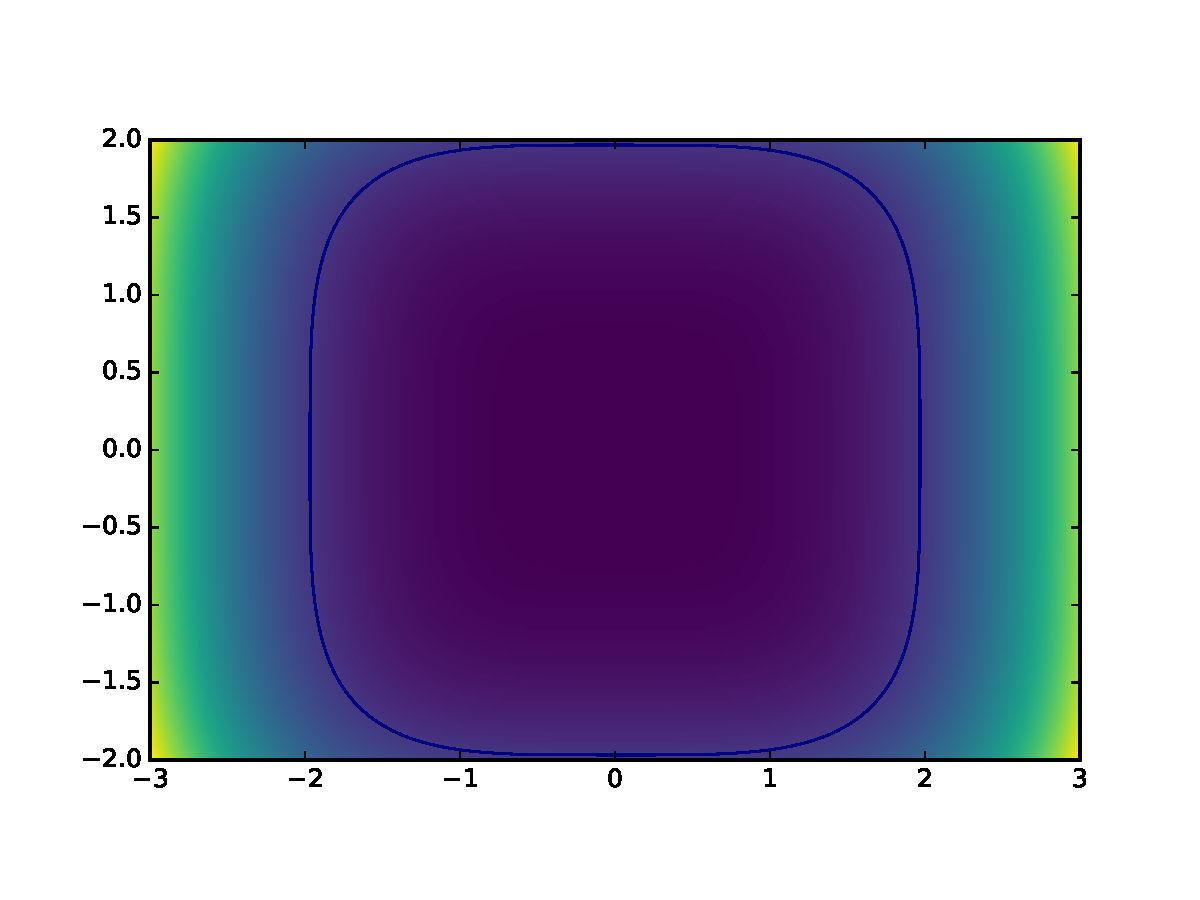
\includegraphics[width=10cm, height=8cm]{img/curva0f1.pdf}
  \caption{Curva de nivel 0 de $F_{1}$.}
  \label{fig:sub1}
\end{subfigure}%
\begin{subfigure}{.5\textwidth}
  \centering
  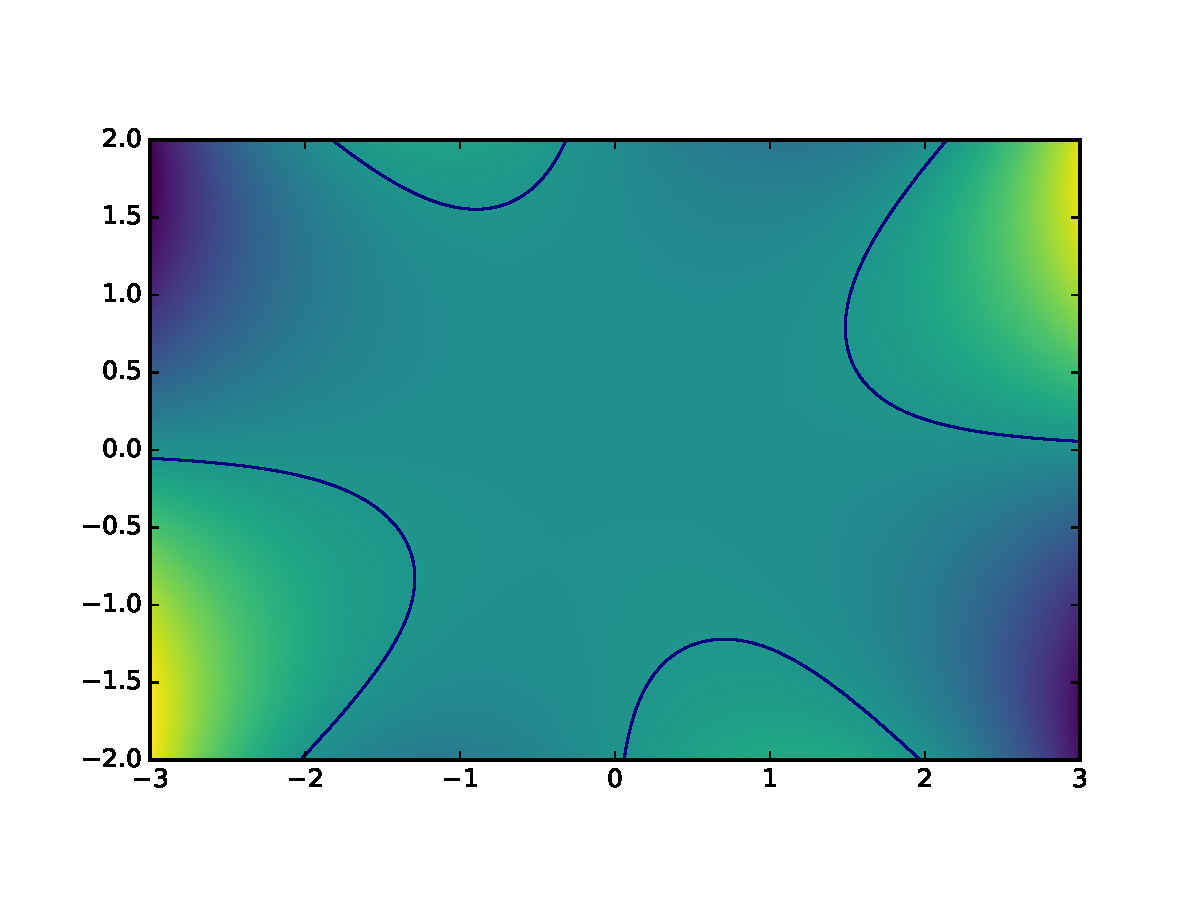
\includegraphics[width=10cm, height=8cm]{img/curva0f2.pdf}
  \caption{Curva de nivel 0 de $F_{2}$.}
  \label{fig:sub2}
\end{subfigure}
\caption{Curvas de nivel 0 de $F_{1}$ y $F_{2}$}
\label{fig:test}
\end{figure}

Para visualizar mejor las intersecciones de ambas curvas se grafican ambas curvas de nivel simult\'aneamente como muestra la figura 2.

\fig{interseccioncurvas.pdf}{15cm}{10cm}{Intersecci\'on de las curvas de nivel 0 de $F_{1}$ y $F_{2}$.} \newpage

Note que la curva de nivel de $F_{1}$ es cerrada, por lo tanto se puede parametrizar con las siguientes expresiones:
\begin{equation}
	x(t) = \sqrt[4]{15}\cdot\text{sign}(\sin(t))\sqrt[4]{\sin^{2}(t)}
\end{equation}
\begin{equation}
	y(t) = \sqrt[4]{15}\cdot\text{sign}(\cos(t))\sqrt[4]{\cos^{2}(t)}
\end{equation}

Luego, s\'olo basta recorrer la curva de $F_{1}$ a lo largo de la parametrizaci\'on dada por las ecuaciones (3) y (4) para encontrar los ceros de $F_{2}$. Dado que la parametrizaci\'on es similar a la de una circunferencia, se hace un s\'imil con una; con esto se propone que el primer cero de la funci\'on, partiendo de $t=0$ est\'a cerca de $\frac{\pi}{4}$, lo cual se corrobora al trazar la parametrizaci\'on como muestra la figura 3. Con esto se elige el primer punto `$a$'. Para elegir el punto `$b$' se le suma un valor delta a `$a$' tal que la curva pase el $0$ de $F_{2}$ y se pueda hacer la bisecci\'on. Esto est\'a ejemplificado en la figura 4. \\ Este proceso se repite para todos los valores $n\frac{\pi}{4}$ con $n = 1\ldots 8$ y con los valores $0.5$ y $-0.5$ para $\delta$ dentro de una funci\'on llamada \textbf{busca\_ceros}.

\fig{contour1.pdf}{15cm}{8cm}{En rojo: trazado de la parametrizaci\'on de la curva de $F_{1}$ desde $t=0$ hasta $t=\frac{\pi}{4}$}
\fig{pi4eps.pdf}{15cm}{8cm}{En rojo: trazado de la parametrizaci\'on de la curva de $F_{1}$ desde $t=0$ hasta $t=\frac{\pi}{4}+\delta$ con $\delta = 0.5$}

\newpage
\section{Resultados}
Los puntos encontrados y las evaluaciones de $F_{1}$ y $F_{2}$ en ellos est\'an presentados en el cuadro 1.
\begin{table}[!ht]
\begin{tabular}{|c|c|c|}
\hline
Puntos $(x,y)$ & $F_{1}(x,y)$ & $F_{2}(x,y)$ \\ \hline
$(1.7669473251533254, 1.5138783340135835)$ & $-1.7763568394002505\text{e-15}$ & $-3.3306690738754696\text{e-15}$ \\ \hline
$(1.9679281913239208, 0.20807043855682616)$ & $-7.105427357601002\text{e-15}$ & $-3.3306690738754696\text{e-15}$ \\ \hline
$(1.6195315294277728, -1.6880897500097491)$ & $-3.552713678800501\text{e-15}$ & $1.687538997430238\text{e-14}$ \\ \hline
$(0.063041119148445249, -1.9679891532205411)$ & $0.0$ & $2.9687363678476686\text{e-13}$ \\ \hline
$(-1.6899275421855853, -1.6174428867372699)$ & $-3.552713678800501\text{e-15}$ & $-2.3092638912203256\text{e-14}$ \\ \hline
$(-1.9679539076104238, -0.18171451675948014)$ & $-7.105427357601002\text{e-15}$ & $-2.646771690706373\text{e-13}$ \\ \hline
$(-1.5040652893171853, 1.7730278324283797)$ & $-3.552713678800501\text{e-15}$ & $-2.708944180085382\text{e-14}$ \\ \hline
$(-0.33068189913134088, 1.9675973488473744)$ & $-7.105427357601002\text{e-15}$ & $1.234568003383174\text{e-13}$ \\ \hline
\end{tabular}
\caption{Tabla con los puntos $(x,y)$ en donde $F_{1} = F_{2} = 0$ con una tolerancia de $10^{-20}$}
\end{table}

\section{Conclusiones}
Se concluye que se encontraron los puntos que hacen cero a ambas funciones simult\'aneamente con una tolerancia de $10^{-20}$

\section{Ap\'endice}
El mensaje escondido en el commit es: `Alo, con la casa de la Cultura? Si, conchetumadre' - N. Parra

\end{document}
